\documentclass[bluish,slideColor,colorBG,pdf]{prosper}
\hypersetup{pdfpagemode=FullScreen}
\usepackage{amsfonts}
\usepackage{amsmath}
\usepackage{graphicx}
\usepackage{color}
\def\baselinestretch{0.7}
\setlength{\topmargin}{-80pt}
\setlength{\textheight}{600pt}
\setlength{\oddsidemargin}{0pt}
\setlength{\evensidemargin}{60pt}
\setlength{\textwidth}{577pt}
\setlength{\footskip}{0pt}
\parindent 0.3in
\hyphenpenalty=10000
\tolerance=10000
\pagestyle{empty}

% expectation symbol -- use "\expect"
\DeclareSymbolFont{AMSb}{U}{msb}{m}{n}
\DeclareMathSymbol{\expect}{\mathalpha}{AMSb}{'105}

\title{Overview: morphometrics and phylogenies}

\author{Joe Felsenstein}
\institution{Bio 550D, Autumn2016}

\begin{document}

{\parindent=0in

\maketitle

\begin{slide}[Replace]{Fred Bookstein is my coteacher in this class}

\begin{center}
\includegraphics[height=1.2in]{Bookstein2009gray.ps}
\end{center}

\centerline{Fred L.Bookstein}

\end{slide}

\begin{slide}[Replace]{A standard quantitative genetics model}

\centerline{\includegraphics[width=4.0in]{quantmodel6.ydraw}}

\end{slide}

\overlays{3}{
\begin{slide}[Replace]{A model of quantitative characters on a phylogeny}

\centerline{\includegraphics[width=2in]{fig23-2.ydraw}}

\begin{itemstep}
\item Brownian motion with multiple characters with different variances and with covariation as well.
\item This started with approximating gene frequencies in the 1960s by
Anthony Edwards and Luca Cavalli-Sforza.
\item I expanded it to model quantitative characters determined by these
geness (1973, 1981, 1988).
\item Assumption that character variances and covariances
are replenished by mutation and do not change much through time.
\item The main person introducing these models was Russ Lande.
\end{itemstep}

\end{slide}
}

\begin{slide}[Replace]{Models for long-term evolution}

\bigskip

The use of quantative genetics approximations to model long-term evolution
in lineages was largely introduced by Russ Lande in the 1980s.
\bigskip

\centerline{\includegraphics[width=2in]{Lande2011.ps}}
\bigskip

Russell Lande, from his website at Imperial College, U.K., where he has been in recent years.

\bigskip

\end{slide}

\overlays{2}{
\begin{slide}[Replace] {Where do the covariances come from? }
\bigskip

\begin{itemstep}
\item {\bf Genetic covariances} (the same loci affect two or more traits).
Genetic drift or natural selection can change the gene frequencies at
these loci, and thus make correlated changes in the two traits.
\item {\bf Selective covariances} (Olof Tedin, 1926; G. Ledyard Stebbins 1950) The 
same environmental conditions can select changes in two or more traits -- even
though they may have no genetic covariance.  This source of evolutionary
covariance is widely ignored.
\end{itemstep}

\end{slide}
}

\begin{slide}[Replace]{How to use morphometric coordinates on phylogenies? }
\bigskip

Is it possible to simply use the coordinates of landmarks
$(x_1, y_1), (x_2, y_2), \dots, (x_p, y_p)$ as continuous
phenotypes $x_1, y_1, \dots, x_p, y_p$  using Brownian motion along a phylogeny?
\bigskip

Yes, but ...
\bigskip

We must do proper morphometrics (correct for translation? rotation?)
\bigskip

\end{slide}

\begin{slide}[Replace]{Can we superpose specimens? }

Consider two cases:

\centerline{\includegraphics[width=3.5in]{superposition.idraw}}
\bigskip

Are these different?
\end{slide}

\begin{slide}[Replace]{Why superposition is in principle impossible}

Consider two cases:

\centerline{\includegraphics[width=3.5in]{superposition.idraw}}
\bigskip

Are these different? ~~ {\Large No!}

\end{slide}

\begin{slide}[Replace]{Dealing with translation}

In effect one is centering each specimen so that
the mean of its points is at $(0, 0)$.  (The
assumption is that the horizontal and vertical
placement of the specimen on the digitizer is
not useful information).
\bigskip

This has the effect of dropping two degrees of
freedom so that each specimen now has $2p-2$
coordinates.  It now ``lives'' in a $(2p-2)$-dimensional
space.
\bigskip

\end{slide}

\begin{slide}[Replace]{The annoying issue of rotation}
\bigskip

\centerline{\includegraphics[width=2.5in]{rotation.idraw}}
\bigskip

Sadly, there is no corresponding transform that
tosses out rotation, as there is for translation.
\bigskip

\end{slide}

\begin{slide}[Replace]{The Procrustes Transform}
\bigskip

\centerline{\includegraphics[width=3in]{procrustes.idraw}}
\medskip

The Procrustes Distance of two forms is the sum of squares of the dashed red
lines (connecting corresponding landmarks).  The forms are superposed
by rotating and translating to minimize this distance.  Generalized Procrustes
Analysis is simply doing rotations and translations to minimize the sum of
squares, summed over all pairs of specimens.


\end{slide}

\begin{slide}[Replace]{The Morphometric Consensus}
\bigskip

\begin{itemize}
\item Superpose (and rescale) specimens by a Generalized Procrustes Transform
\item Compute (square root of) sum-of-squares distances between all of them
\item Get Principal Coordinates from this distance matrix
\item Make a space with these PCs as axes, put points in it, one per specimen.
\end{itemize}

Problems: (1) ignores phylogeny, (2) implicitly assumes that the model of statistical
error is independent, isotropic noise at all landmarks

\end{slide}

\begin{slide}[Replace]{Why you should not ignore phylogenies}
\bigskip

\centerline{
\includegraphics[width=2.5in]{comparative.idraw}}

In inferring means (ancestors), variances and covariances, treating the
species as i.i.d. independent samples ignores that some are near-duplicates
of others.  This is the classical phylogenies-and-the-comparative-method
problem.

\end{slide}

\begin{slide}[Replace]{The ``Pinocchio effect'' }
\bigskip

\centerline{\includegraphics[height=2in]{pinocchio1.idraw}}

If we have a form for which one part (in this case the nose) changes
much more than others, this violates the implicit model of the
Procrustes superposition.

\end{slide}

\begin{slide}[Replace]{The ``Pinocchio effect'' }
\bigskip

\centerline{\includegraphics[height=2in]{pinocchio2.idraw}}

... and a Procrustes superposition that does not take this into
account will tend to overreact to the changes of that part of the form.

\end{slide}

\begin{slide}[Replace]{The ``Pinocchio effect'' }
\bigskip

\centerline{\includegraphics[height=2in]{pinocchio3.idraw}}

... whereas a more sensible approach would allow that point to deviate
farther because it changes more readily.

\end{slide}

\begin{slide}[Replace]{Removing translation and rotation}
\bigskip

\begin{itemize}
\item We remove translation by centering each specimen on (0, 0), which
drops 2 degrees of freedom in a two-dimensional space.
\item We remove rotation by estimating each specimen's rotation angle
by maximizing the log-likelihood for the whole study with respect to
it.  (Keep rotating them each until the overall log-likelihood is maximum).
\item There is something similar that can be done to separate size and shape.
\end{itemize}

\end{slide}

\begin{slide}[Replace]{Instead of the ``morphometric consensus'' }
\bigskip

... we do {\it not} do the usual Procrustes distances and PCs in
the tangent space.  That implicitly assumes equal and independent
noise in each coordinate.
\bigskip

Instead we assume a multivariate Brownian Motion with arbitrary
evolutionary covariances, and we estimate them, just as one does
in phylogenetic comparative methods.

\end{slide}

\begin{slide}[Replace]{Our method is similar but uses phylogenies}
\bigskip

\begin{itemize}
\item We compute the likelihood of changes on a phylogeny using
a (covarying) Brownian motion model
\item We are maximizing the likelihood to infer the covariance matrix
\item We do superpose the centroids of the specimens, just as the MMC does.
\item The rotations are chosen, iteratively, specimen by specimen, to maximize the likelihood
\item We are in effect using the phylogenetically independent contrasts on the
tree instead of treating the specimens as independent data
\end{itemize}
\bigskip

Basically, none of the steps of the Morphometric Consensus are left
except for centering all specimens at their centrois.

\end{slide}

\begin{slide}[Replace]{A simulation test}
{\ptsize{8}
\begin{enumerate}
\itemsep -3pt
\item Generate 50 100-species trees by a pure birth process
\item For each evolve 100 forms by (covarying) Brownian Motion up the
tree
\item These are the true covariances:
\end{enumerate}

\centerline{\includegraphics[width=2.2in]{urfish2.idraw}}

\begin{itemize}
\itemsep -3pt
\item All 10 landmarks move by independent and equal Brownian Motion of the
coordinates with variance (per unit branch length) of 0.001, {\it plus}
\item the vertical coordinate of the pectoral fin and the two coordinates
of the top of the tail move in a perfectly correlated change with variance
0.003.
\end{itemize}

}
\end{slide}

\begin{slide}[Replace]{The true tree for one of the 100 data sets}
\bigskip

\centerline{\includegraphics[width=3in]{truetree.idraw}}

\end{slide}

\begin{slide}[Replace]{20 of the 100 fishes from data set \#2, centered and rotated}
\bigskip

\centerline{\includegraphics[width=3in]{fishes28.2.idraw}}

\end{slide}

\begin{slide}[Replace]{20 of the 100 fishes from data set \#2, also rescaled}
\bigskip

\centerline{\includegraphics[width=3in]{fishes28.2shape.idraw}}

\end{slide}

\begin{slide}[Replace]{First PC 1 for data set \#2}
\bigskip

\centerline{\includegraphics[width=3in]{fishes28.2.formandpc.idraw}}
\bigskip

This principal component shows both size changes and the fin extensions,
and it is not easy to see which is which.

\end{slide}

\begin{slide}[Replace]{First shape PC 1 for data set \#2}
\bigskip

\centerline{\includegraphics[width=3in]{fishes28.2shape.formandpc.idraw}}
\bigskip

Now we've inferred a scale (size) component and removed it from the
covariances, and then taken the first PC of the residual on size.  We
can see the fin component more clearly.

\end{slide}

\begin{slide}[Replace]{Making the first shape PC sparser by ``medianizing'' }
\bigskip

\centerline{\includegraphics[width=3in]{fishes28.2shape.formandpcmed.idraw}}
\bigskip

To make PC1 be sparses we can add in a little location (not forcing the
changes to maintain the centroid supeposition).  This is done by subtracting
from the $\mathsf{~x~}$ components, their median, and similarly for the
$\mathsf{~y~}$ components.  So it minimizes the $\mathsf{L^1}$ norm of the
PC coefficients.

The result is very clear.

\end{slide}

\begin{slide}[Replace]{What do we get from the Morphometric Consensus? }

Using a Procrustes superposition and assuming the forms are i.i.d. and then
computing principal components:
\medskip

\centerline{\includegraphics[width=3in]{fishes28.2proc.formandpc.idraw}}

... we get a not-as-clear result with some size still there -- we have ignored the tree and taken out size by standardizing centroid size, which is affected more by the fin component in the MMC methods.

\end{slide}

\begin{slide}[Replace]{References}

{~~}\hspace{25pt}\parbox[t]{4in}{\parindent=-15pt

Lande, R.  1976.  Natural selection and random genetic drift in phenotypic
evolution.  {\it Evolution} {\bf 30 (2):} 314-334. \textcolor{purple}{\bf [One
of Russ's major papers using the constant-variances approximation]}

Stebbins, G. L.  1950. Variation and Evolution in Plants.  Columbia University
Press, New York. \textcolor{purple}{\bf [Describes selective covariance and
cites Tedin (1926) for it]}

Felsenstein, J.  1988.  Phylogenies and quantitative characters.  
{\it Annual Review of Ecology and Systematics} {\bf 19:} 445-471. \textcolor{purple}{\bf [Review]}

Felsenstein, J.  2002.  Quantitative characters, phylogenies, and morphometrics.pp. 27-44 in ``Morphology, Shape, and Phylogenetics", ed. N. MacLeod.
Systematics Association Special Volume Series 64.  Taylor and Francis, London.
\textcolor{purple}{\bf [Review repeating 1988 material.]}

Felsenstein, J.  2004.  {\it Inferring Phylogenies.}  Sinauer Associates,
Sunderland, Massachusetts.
\medskip

}
\vfill

\end{slide}
}

\end{document}

